%!TEX root = ../thesis.tex
% appendix section 5

\chapter{Laser pulse energy measurement}
\label{sec:ap5}

\begin{figure}[ht!]
\centering
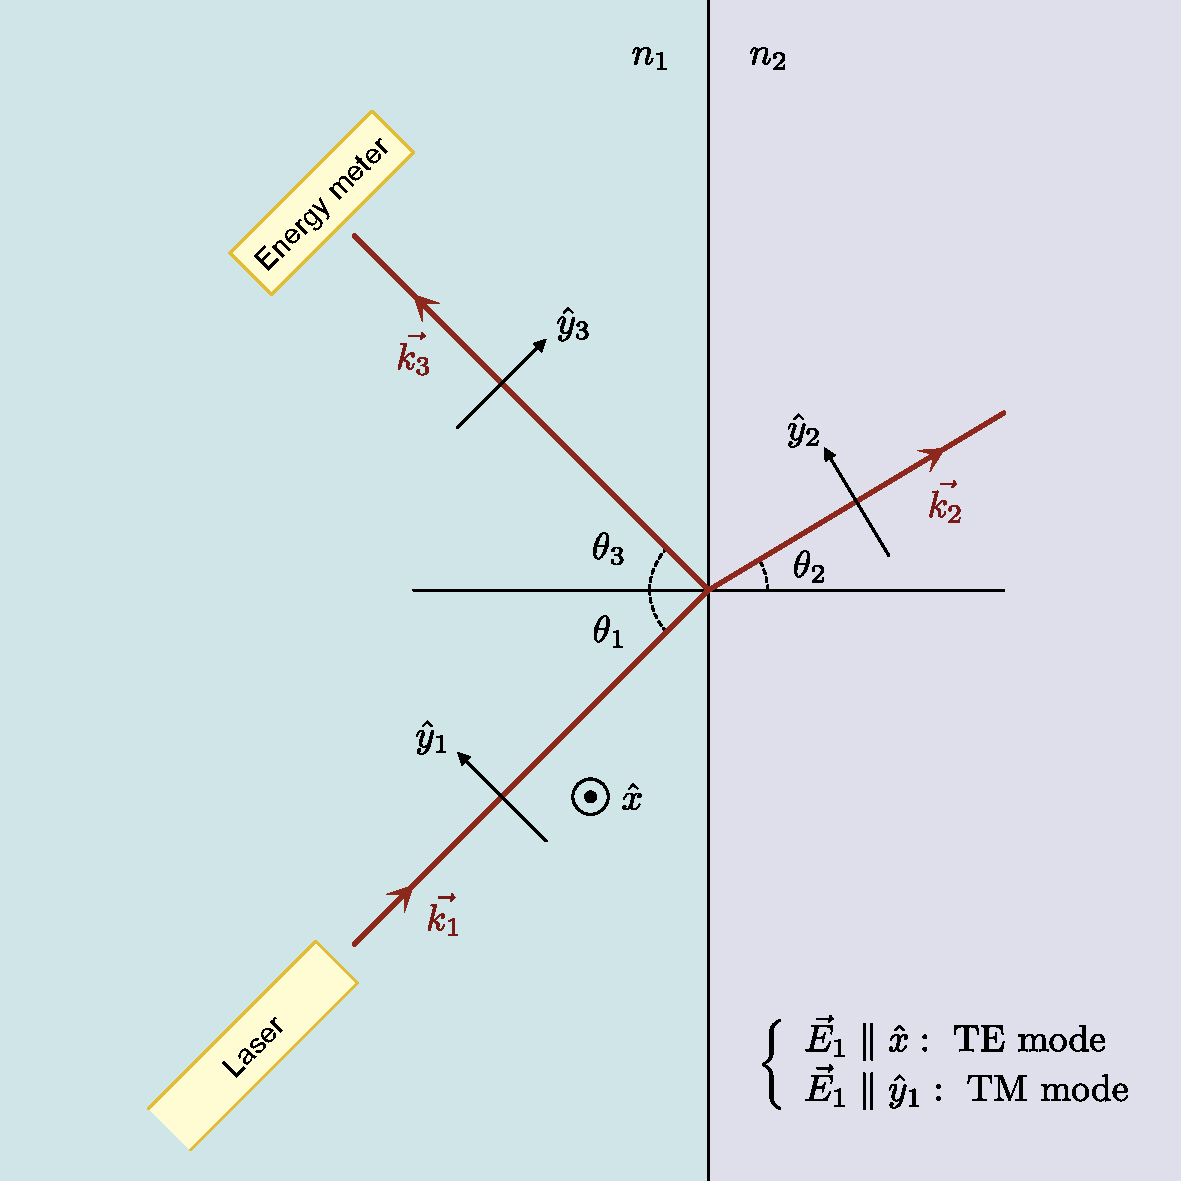
\includegraphics[width=100mm]{figures/ap5/Fresnel/Fresnel.pdf}
\caption{Plane of incidence and coordinates. Transverse electric field (TE) mode is when the polarization of incident light ($\vec{E}_1$) is vertical to the plane of incidence. On the other hand, transverse magnetic field (TM) mode is when the polarization is parallel to the plane. The intensity of the reflected and refracted light may change by varying the incident angle.}
\label{fig:Fresnel}
\end{figure}

Due to the intense pulse energy, the direct energy measurement of the laser requires a solid detector. We used a simple method to bypass this difficulty. We can determine the pulse energy by measuring the angle dependence of the reflected energy by a thin glass with a known refractive index (a plane of incidence and coordinates are illustrated in Fig.\ref{fig:Fresnel}). The transmittance and the reflectance of the laser energy depend on the polarization of the incident light and are described by the Fresnel equation (Chap.6 in \cite{saleh2019fundamentals})
\begingroup
\allowdisplaybreaks
\begin{align}
R_\text{TE} \left( \theta_1 \right) &= \abs{ \frac{n_1 \cos \left( \theta_1 \right) - n_2 \cos \left( \theta_2 \right)}{n_1 \cos \left( \theta_1 \right) + n_2 \cos \left( \theta_2 \right)} }^2 \\
R_\text{TM} \left( \theta_1 \right) &= \abs{ \frac{ - n_1 \sec \left( \theta_1 \right) + n_2 \sec \left( \theta_2 \right)}{n_1 \sec \left( \theta_1 \right) + n_2 \sec \left( \theta_2 \right)} }^2
\end{align}
\endgroup
, where the subscript TE (TM) stands for the transverse electric (magnetic) field, $n_{1(2)}$ and $\theta_{1(2)}$ are the refractive index of the medium 1 (2) and the incident (refracted) angle. Due to the real world alignment, the polarization may be blended even we setup vertical polarization (TE), and thus, the model for the reflected energy becomes
\begin{equation}
\mathcal{E}_\text{meas} = \left[ \alpha R_\text{TE} + \left( 1-\alpha \right) R_\text{TM} \right] \mathcal{E}_\text{laser}
\end{equation}
Using the known values for air $n_1 \approx 1$ and for sodalime glass $n_2 \approx 1.513$ together with the Snell's law reduces the above model equation as a function of incident angle $\theta_1$ leaving $\alpha$ and $\mathcal{E}_\text{laser}$ as the fitting parameters. The result of the measurement is shown in Fig.\ref{fig:pulseEnergy}.

\begin{figure}[ht!]
\centering
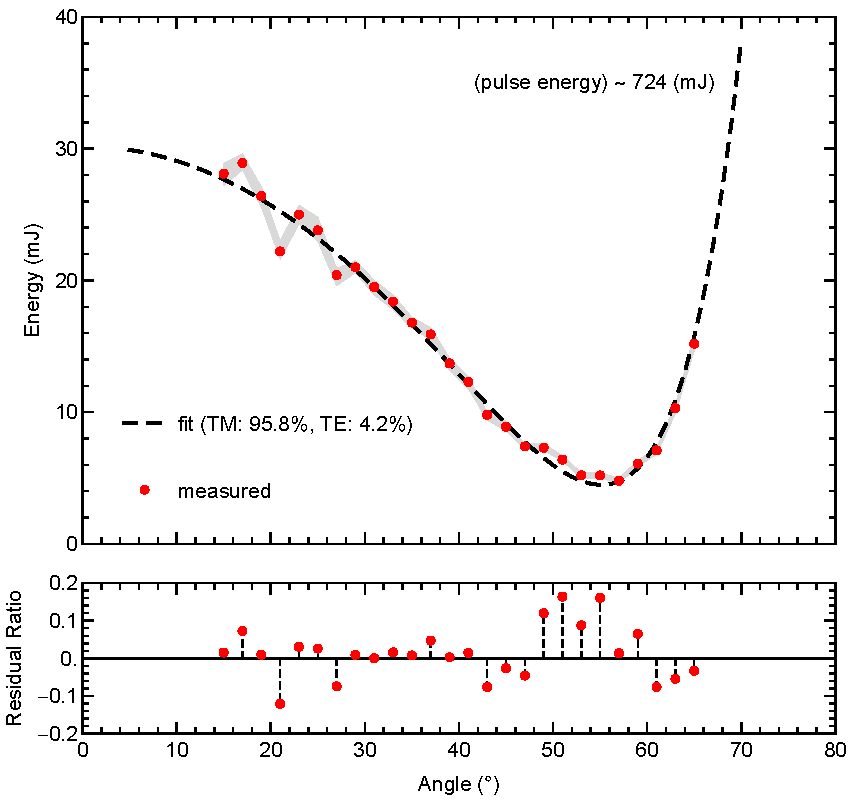
\includegraphics[width=100mm]{figures/ap5/pulse/energy.pdf}
\caption{Pulse energy measurement of the intense laser with the help of a glass reflection model. The measured pulse energy is about $720 \text{ mJ/pulse}$.}
\label{fig:pulseEnergy}
\end{figure}


